\chapter{Exploration} \label{chap:explor}

\section{Introduction} \label{sec:explor:intro}
The previous chapter listed existing interaction techniques combining AR, feedforward and ubicomp. We will now perform our own exploratory study of the design space. The results of this study will help us focus the remainder of our research and prepare for a more high-fidelity experiment in the next chapter. We will base our exploration on an online survey, since it allows for a large number of participants in a short amount of time. See Appendix \ref{chap:explor_survey} for a full printout of the survey, including the introductory information that participants received.

\section{Survey} \label{sec:explor:survey}
    \subsection{Procedure} \label{subsec:explor:survey:procedure}
    We aim to investigate for a range of interaction techniques how well they work in different ubicomp setups. We achieve this by having the participants try out a set of scenarios and rate them on various aspects. Each of these scenarios will have some problem that the participants must try to solve. Some will be baseline scenarios where the participants receive no help, but most will be augmented scenarios where the participants are aided in their task by some form of AR feedforward that we wish to evaluate.

    Since our survey targets the general population, AR and ubicomp may be foreign concepts to some participants, and thus we must take special care not to confuse or overwhelm them. We also prefer the setups to offer problems that the participants have encountered before, helping them to understand the task and stimulating them. For this reason, we opted to focus on the problem of mapping light switches to their corresponding lights. This is a recognizable and conceptually simple problem, but still allows for setups of arbitrary complexity.
    
    Our next question is how many and which setups to choose. Ideally, we would use only one setup for all scenarios, to eliminate an extra variable from our experiment. A second reason to limit the number of setups is that for each setup we must add a baseline scenario without feedforward to compare the other scenarios against. However, the set of possible setups is extremely diverse. A symmetric rectangular hall with a grid of lights on the ceiling might benefit most from different approaches than a cozy lounge with various lights on walls and tables. We could test each approach in multiple setups, but this would reduce the number of approaches we could include.
    
    We decide on using two setups, which limits the number of baselines, but still allows for some variety in the scenarios. We will test each feedforward approach only in the setup in which we expect it to work best, to maximize the number of approaches that we can investigate. This choice reflects the preliminary nature of this study. The promising approaches can still be investigated further in a follow-up study. Both of the chosen setups are of moderate complexity, to create scenarios that challenge our approaches but that one might still encounter in day-to-day life. 
    
    The first setup is the ``Kitchen'', shown in Scenario 1 in Appendix \ref{chap:explor_survey}. It is a picture we found online \cite{FileTROY82:online}. This room has a variety of wall, hanging and ceiling lights, six in total. There are four light switches, one larger than the rest, arranged in two rows. This setup is meant to be the more complex of the two. We chose it because we believe there is no single obvious mapping of switches on lights. We might create matches based on similar locations, sizes, or some other metric, but in many cases these metrics will contradict each other. This conflict is intentional, as it allows us to determine which metrics the participants will choose over others.
    
    The second setup is the ``Classroom'', a highly symmetric setup comprised of a rectangular room with a 3x3 grid of lights on the ceiling and a row of 3 switches, one large and two small, next to the door. This room does actually exist, and \todo{Still quite a bit to write here.}

    \subsection{Apparatus} \label{subsec:explor:survey:apparatus}
    The survey was created and hosted using Google Forms. It was made available via several online media for the duration of one week, from 2017-11-08 until 2017-11-15. We estimate the average completion time at 20 minutes.

    \subsection{Participants} \label{subsec:explor:survey:participants}
    The survey received a total of 36 unpaid responses. After careful consideration, we chose to discard two responses. In the first discarded submission, the participant wrote that they could not answer some questions due to technical difficulties, and in the second, the participant's commentary clearly showed that they had misunderstood some questions. Our results and analysis are thus based on 34 responses, with demographics as shown in Table \ref{table:explor:demographics}. The average age of the participants was 27 years.

        \begin{table}[h!]
        \centering
            \begin{tabular}{|c|c c|c|} 
            \hline
                      & Male & Female &    \\
            \hline
            Age 17-25 &   18 &      8 & 26 \\
            Age 33-53 &    5 &      3 &  8 \\
            \hline
                      &   23 &     11 & 34 \\
            \hline
            \end{tabular}
        \caption{Demographics}
        \label{table:explor:demographics}
        \end{table}

\section{Results} \label{sec:explor:results}

\section{Discussion} \label{sec:explor:discussion}
\todo{This work in progress is still a mix of results and discussion, it must be split up.}
We start off by discussing the two baseline scenarios. The first question we wanted to ask ourselves after closing the survey was ``What is the most common solution for each scenario, and how common is it?''. In other words, we want to know whether a consensus is reached, or if there is total disagreement among respondents. Figures \ref{fig:preliminary_study_kitchen_baseline_consensus} and \ref{fig:preliminary_study_classroom_baseline_consensus} show the most common solution for both baseline scenarios, by putting the labels of connected lights and switches in the same color. The consensuses are also summarized in table \ref{table:preliminary_study_consensus}.

\begin{figure}
    \centering
    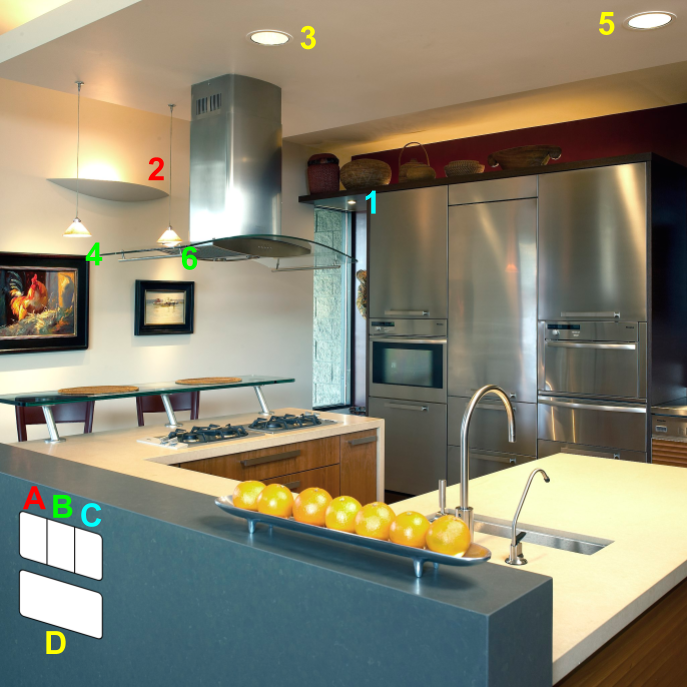
\includegraphics[width=0.7\linewidth]{exploration/kitchen_baseline_consensus.png}
    \caption{Kitchen baseline consensus}
    \label{fig:preliminary_study_kitchen_baseline_consensus}
\end{figure}

\begin{figure}
    \centering
    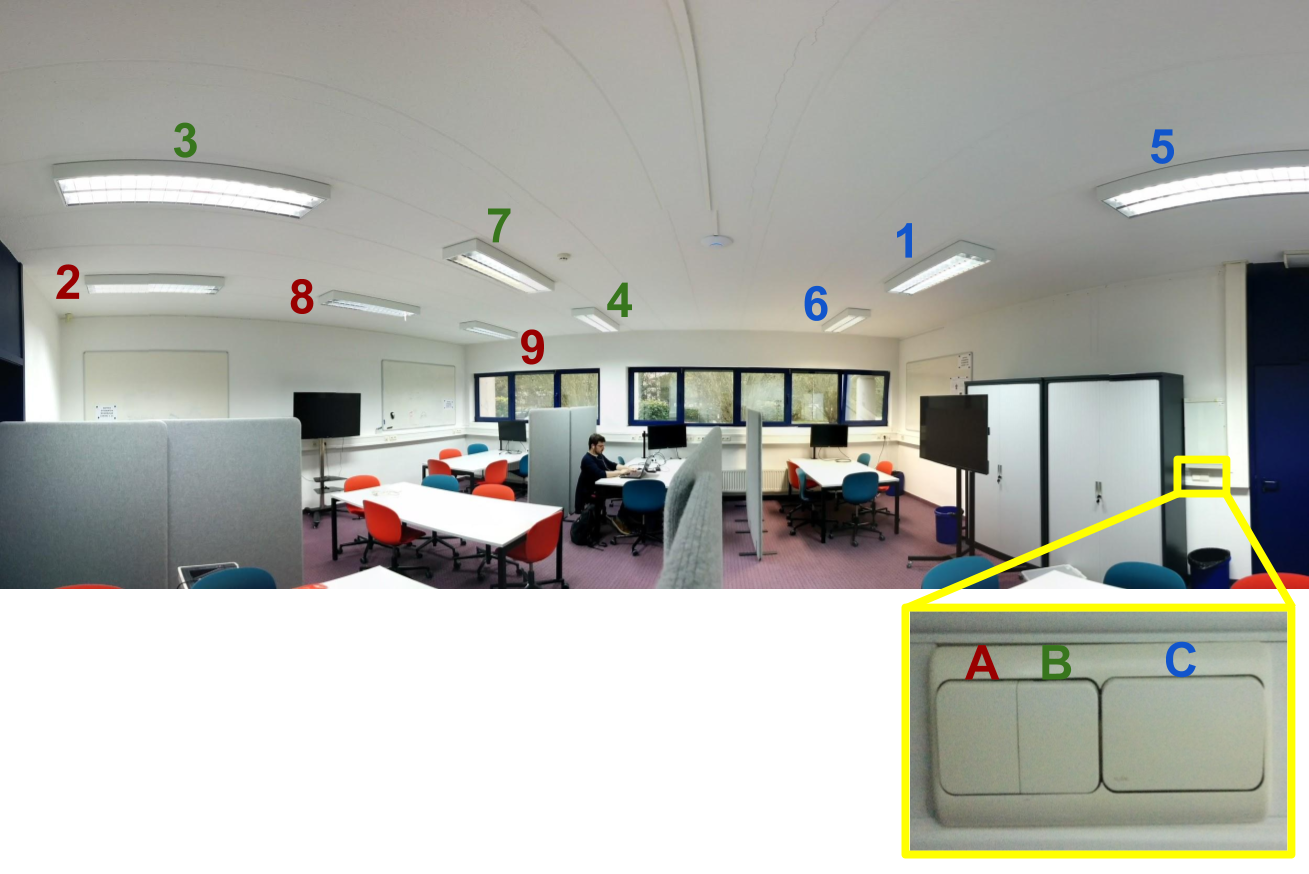
\includegraphics[width=1.0\linewidth]{exploration/classroom_baseline_consensus.png}
    \caption{Classroom baseline consensus}
    \label{fig:preliminary_study_classroom_baseline_consensus}
\end{figure}

\begin{table}[h!]
    \centering
    \begin{tabular}{|c|c|c|} 
    \hline
      & Kitchen & Classroom \\
    \hline
    A & 2       & 2, 8, 9   \\
    B & 4, 6    & 3, 7, 4   \\
    C & 1       & 1, 5, 6   \\
    D & 3, 5    & N/A       \\
    \hline
\end{tabular}
\caption{Baseline scenario consensuses}
\label{table:preliminary_study_consensus}
\end{table}

For the kitchen scenario, the most common solution was given by 10 out of 34 respondents, or 29.41\%. In total, 20 different solutions were offered. We believe this shows strong disagreement, since no configuration would be intuitive for even a third of the respondents. For the classroom scenario, the most common solution was given by 21 out of 34 respondents, or 61.76\%. In total, 9 different solutions were offered. We believe this shows a clear consensus, but is still problematic because no matter the configuration, at least one in three respondents would find it confusing.

Next we wanted to know the rationale behind the given solutions. In the survey, seven assumptions were provided, and for each of them, the respondent had to indicate whether it played ``no role'', a ``small role'' or a ``large role'' in determining their solution. The results can be seen in Figure \ref{fig:preliminary_study_rationales}. In this bar chart, we awarded one point to an assumption each time a respondent indicated it played a ``large role'', half a point if it played a ``small role'' and no points if it played ``no role''. For example, an assumption with ten points may have played a ``large role'' eight times and a ``small role'' four times.

\begin{figure}
    \centering
    \def\svgwidth{\columnwidth}
    \import{resources/exploration/figures/}{rationales.pdf_tex}
    \caption{Rationales in baseline scenarios}
    \label{fig:preliminary_study_rationales}
\end{figure}

Our first conclusion from Figure \ref{fig:preliminary_study_rationales} is that respondents clearly based their solutions in the kitchen scenario on three main assumptions, which are, in descending order:

\begin{enumerate}
    \item Each switch controls the lights that are closest to it.
    \item Larger switches control larger lights.
    \item Larger switches control more lights.
\end{enumerate}

When looking back at the consensus in Figure \ref{fig:preliminary_study_kitchen_baseline_consensus}, we do indeed find these three assumptions. A testimony to the first assumption is the fact that the leftmost switch A controls the leftmost wall light, the central switch B controls the more centrally placed hanging lights, and the rightmost switch C controls the rightmost (at least from the given viewpoint) small light in the back. The other two assumptions are found in the fact that the large switch D controls the two large ceiling lights, giving it on average more and larger lights than the other switches. The four remaining assumptions are not apparent in the consensus. For example, it is not true that higher placed switches on average control more lights.

\todo{Talk about tendency to group similar lights, and quote remarks by respondents.}

If we now look at the classroom scenario in Figure \ref{fig:preliminary_study_rationales}, we find that the consensus is now strongly based on the single assumption that ``Each switch controls the lights that are closest to it.'', with all other assumptions falling far behind. We believe this happens because the respondent is now given three switches to control a 3x3 grid of identical lights, and so the most straightforward solution is to connect each switch with the row or column of lights that is closest to it, with no other factors taken into consideration. We note that in the consensus the lights are matched to the close-up of the switches, rather than to the actual switches in the room, which are turned 90 degrees. However, we believe that this phenomenon is due to the perspective of the image confusing the respondents, that it would not occur in the real world, and thus that it does not undermine our conclusion.

The third and last topic on the baseline scenarios we want to discuss is the certainty of the respondents. More specifically, we want to compare the certainty of those who followed the consensus to those who did not. For this we created Table \ref{table:preliminary_study_baseline_certainties}. In this table, we can see that the average certainty was slightly higher among respondents who followed the consensus than among those who did not, and was also higher in the classroom scenario than in the kitchen scenario (remember that certainty was indicated by the respondent on a Likert-scale from 1 to 5). However, we believe the main takeaway from this table is that the respondents felt generally uncertain, since no average certainty reached even the middle score of 3 out of 5.

Our main conclusions from the baseline scenarios are as follows. There is much disagreement on the most intuitive configuration in any given scenario. Respondents often feel uncertain when confronted with unfamiliar scenarios, even when they are of simple to average complexity. When presented with an unfamiliar scenario, respondents will typically try to solve it by using the switches as a floor plan. They will try to match the layout of the switches to the layout of the lights, and larger switches will be assigned more or larger lights if it does not conflict with the layout. However, a significant portion of the respondents reasons differently, and thus there is not always a configuration that fits everyone.

\begin{table}[h!]
    \centering
    \begin{tabular}{|c|c c|c|} 
    \hline
              & Followed consensus & Did not follow consensus &      \\
    \hline
    Kitchen   &               2.70 &                     2.21 & 2.35 \\
    Classroom &               2.76 &                     2.54 & 2.68 \\
    \hline
              &               2.73 &                     2.36 & 2.52 \\
    \hline
\end{tabular}
\caption{Average certainty in baseline scenarios}
\label{table:preliminary_study_baseline_certainties}
\end{table}

\subsection{Augmented Scenarios} \label{sec:preliminary_study:augmented_scenarios}

Probably the most obvious question to ask about the augmented scenarios is what percentage of respondents answered correctly for each visualization. The answer to this question can be seen in Figure \ref{fig:preliminary_study_correctness}. This figure includes the baseline scenarios, where a correct solution is considered a solution that follows the consensus. One of the first things to notice here, is that every single visualization scored better results than the baseline scenarios, although the \textit{arcs} did only marginally so. Still, \textit{arcs} and \textit{lines} were both tested in the kitchen scenario, so the margin is much larger when compared to their own baseline. As for the best visualizations, every single respondent answered correctly for \textit{colors}, and \textit{switches on lights} is a close second with only one incorrect solution.

\begin{figure}
    \centering
    \def\svgwidth{\columnwidth}
    \import{resources/exploration/figures/}{correctness.pdf_tex}
    \caption{Correct solutions per scenario}
    \label{fig:preliminary_study_correctness}
\end{figure}

The next thing we want to do is compare the number of correct solutions to the certainty that respondents indicated. The certainty per scenario can be seen in Figure \ref{fig:preliminary_study_certainties}, which again includes the baseline scenarios. Here we see that the \textit{arcs} barely offer any improvement over their baseline scenario; respondents still feel very uncertain when using them, even though their solutions are much more often correct. We also see that respondents are less certain when using the \textit{hovering floor plan} than when using \textit{lines}, even though they gave more correct solutions. The remaining four visualizations all have both a hight number of correct solutions and a high certainty.

\begin{figure}
    \centering
    \def\svgwidth{\columnwidth}
    \import{resources/exploration/figures/}{certainties.pdf_tex}
    \caption{Certainty per scenario}
    \label{fig:preliminary_study_certainties}
\end{figure}

We will now look at the subjective experience of the respondents. The results of the five Nielsen dimensions that we used can be seen in Figures \ref{fig:preliminary_study_easy_to_learn}, \ref{fig:preliminary_study_fast_to_work_with}, \ref{fig:preliminary_study_resistant_to_errors}, \ref{fig:preliminary_study_useful} and \ref{fig:preliminary_study_enjoyable}. A first thing to notice is that the top three in all five dimensions is the same: first \textit{colors}, second \textit{switches on lights} and third \textit{lights on switches}.

\begin{figure}
    \centering
    \def\svgwidth{\columnwidth}
    \import{resources/exploration/figures/}{easy_to_learn.pdf_tex}
    \caption{``Easy to learn'' scores per scenario}
    \label{fig:preliminary_study_easy_to_learn}
\end{figure}

\begin{figure}
    \centering
    \def\svgwidth{\columnwidth}
    \import{resources/exploration/figures/}{fast_to_work_with.pdf_tex}
    \caption{``Fast to work with'' scores per scenario}
    \label{fig:preliminary_study_fast_to_work_with}
\end{figure}

\begin{figure}
    \centering
    \def\svgwidth{\columnwidth}
    \import{resources/exploration/figures/}{resistant_to_errors.pdf_tex}
    \caption{``Resistant to errors'' scores per scenario}
    \label{fig:preliminary_study_resistant_to_errors}
\end{figure}

\begin{figure}
    \centering
    \def\svgwidth{\columnwidth}
    \import{resources/exploration/figures/}{useful.pdf_tex}
    \caption{``Useful'' scores per scenario}
    \label{fig:preliminary_study_useful}
\end{figure}

\begin{figure}
    \centering
    \def\svgwidth{\columnwidth}
    \import{resources/exploration/figures/}{enjoyable.pdf_tex}
    \caption{``Enjoyable'' scores per scenario}
    \label{fig:preliminary_study_enjoyable}
\end{figure}
